\usetikzlibrary{positioning,fit}
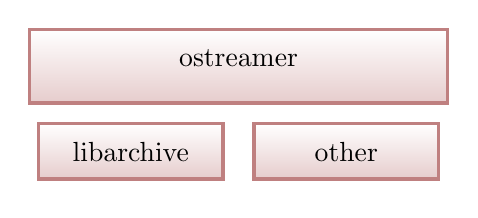
\begin{tikzpicture}[
  phantom/.style={
    rectangle,
    draw=red,
    text width=6em,
    %inner sep=1em,
    outer sep=0em,
    minimum height=2em
  },
  block/.style={
    rectangle,
    very thick,
    draw=red!50!black!50,
    top color=white,
    bottom color=red!50!black!20,
    text width=6em,
    %inner sep=1em,
    outer sep=0em,
    minimum height=2em,
    text centered
  },
  blockn/.style ={rectangle,text width=6em,draw,minimum height=3em, outer sep=0pt},
  phantomn/.style ={rectangle,text width=6em,minimum height=3em, outer sep=0pt}]
  \matrix[column sep=1em, row sep=1em]
 {
  % first row
  \node[phantom] (ost0) {}; & \node[phantom] (ost1) {}; \\
  % second row
  \node[block] (libarchive) [] {libarchive}; & \node[block] (other) [] {other}; \\
  };
  \node[block] (ostreamer) [fit=(ost0) (ost1)] {ostreamer};
\end{tikzpicture}
% http://tex.stackexchange.com/questions/58048/tikz-node-covering-several-columns